\exercise

Let us given the binary strings $S = \{ 0001100, 0001110, 0011, 0010, 101, 111
\}$.
%
\begin{enumerate}
  \item Show the compacted trie for $S$.
  \item Show the Patricia trie for $S$.

  \item Assuming that $S$ is on disk and the compacted trie is in internal memory,
  with edge labels implemented via pointers to substrings of $S$, show the
  I/O-complexity of prefix-searching for a pattern $P[1, p]$.

  \item Assuming that $S$ is on disk and the Patricia trie is in internal memory,
  with leaf pointers to strings of $S$, show the I/O-complexity of
  prefix-searching for a pattern $P[1, p]$.

  \item Show how to search in the Patricia trie for the lexicographic position
  of $P_1 = 010000$, and of $P_2 = 0101$.

\end{enumerate}

\solution

\begin{itemize}

  \item[1, 2.] \autoref{fig:tries} shows the graphical representation of the
  compacted trie and Patricia trie.
  %
  \begin{figure}[t]
    \begin{subfigure}{0.5\textwidth}
      \centering
      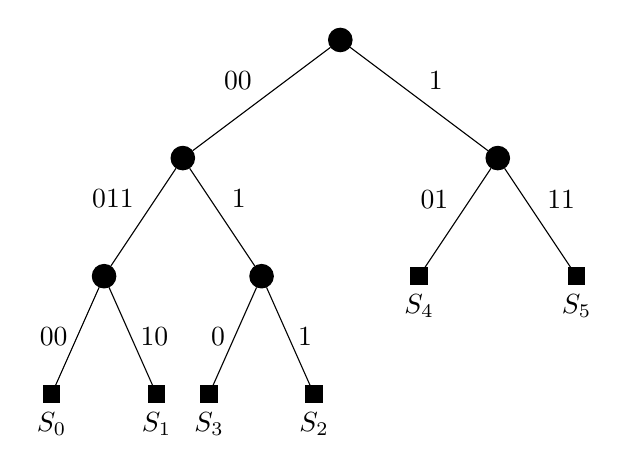
\begin{tikzpicture}[
        grow=down,
        inner/.style={draw, fill=black, inner sep=3, circle},
        leaf/.style={draw, fill=black, inner sep=3},
        level/.style={sibling distance = 4cm/#1, level distance = 1.5cm}
      ]
      \node[inner] {}
          child {
              node[inner] {}
              child {
                  node[inner] {}
                  child {
                      node[leaf, label=below:$S_0$] {}
                      edge from parent[-] node[left] {00}
                  }
                  child {
                      node[leaf, label=below:$S_1$] {}
                      edge from parent[-] node[right] {10}
                  }
                  edge from parent[-] node[above left] {011}
              }
              child {
                  node[inner] {}
                  child {
                      node[leaf, label=below:$S_3$] {}
                      edge from parent[-] node[left] {0}
                  }
                  child {
                      node[leaf, label=below:$S_2$] {}
                      edge from parent[-] node[right] {1}
                  }
                  edge from parent[-] node[above right] {1}
              }
              edge from parent[-] node[above left] {00}
          }
          child {
              node[inner] {}
              child {
                  node[leaf, label=below:$S_4$] {}
                  edge from parent[-] node[above left] {01}
              }
              child {
                  node[leaf, label=below:$S_5$] {}
                  edge from parent[-] node[above right] {11}
              }
              edge from parent[-] node[above right] {1}
          };
      \end{tikzpicture}
      \caption{}
    \end{subfigure}
      \begin{subfigure}{0.5\textwidth}
        \centering
        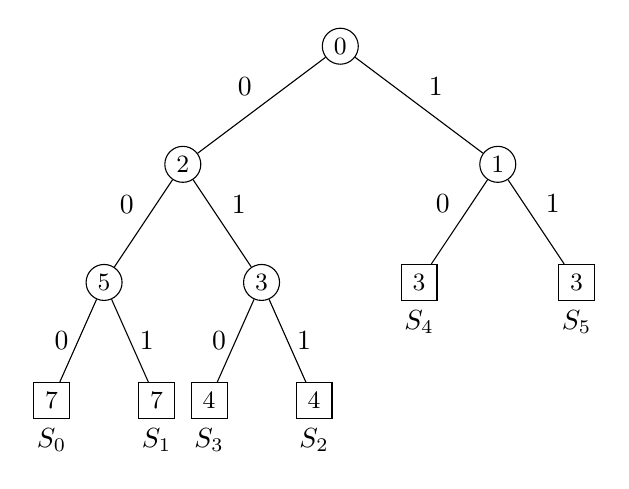
\begin{tikzpicture}[
          grow=down,
          inner/.style={draw, fill=white, inner sep=0, minimum size=13, circle},
          leaf/.style={draw, fill=white, inner sep=0, minimum size=13},
          level/.style={sibling distance = 4cm/#1, level distance = 1.5cm}
        ]
        \node[inner] {\small 0}
            child {
                node[inner] {\small 2}
                child {
                    node[inner] {\small 5}
                    child {
                        node[leaf, label=below:$S_0$] {\small 7}
                        edge from parent[-] node[left] {0}
                    }
                    child {
                        node[leaf, label=below:$S_1$] {\small 7}
                        edge from parent[-] node[right] {1}
                    }
                    edge from parent[-] node[above left] {0}
                }
                child {
                    node[inner] {\small 3}
                    child {
                        node[leaf, label=below:$S_3$] {\small 4}
                        edge from parent[-] node[left] {0}
                    }
                    child {
                        node[leaf, label=below:$S_2$] {\small 4}
                        edge from parent[-] node[right] {1}
                    }
                    edge from parent[-] node[above right] {1}
                }
                edge from parent[-] node[above left] {0}
            }
            child {
                node[inner] {\small 1}
                child {
                    node[leaf, label=below:$S_4$] {\small 3}
                    edge from parent[-] node[above left] {0}
                }
                child {
                    node[leaf, label=below:$S_5$] {\small 3}
                    edge from parent[-] node[above right] {1}
                }
                edge from parent[-] node[above right] {1}
            };
        \end{tikzpicture}
        \caption{}
      \end{subfigure}
    \caption{Graphical representation of
    {\bf (a)} the compacted trie and {\bf (b)} the Patricia trie.}
    \label{fig:tries}
  \end{figure}

  \item[3.] The compact trie solves the prefix-search problem in $O(p +
  n_{occ}/B)$ I/Os, where $n_{occ}$ is the number of strings prefixed by $P$.

  \item[4.] The Patricia trie solves the prefix-search problem in $O(p/B +
  |s|/B\epsilon)$ I/Os, where $s$ is the ``interesting string'' determined by
  the first stage of Blind search, while $\epsilon$ is the parameter regulating
  the space/time trade-off of the Locality-Preserving Front Coding.

  \item[5.] The lexicographic searches are done as follows:
  %
  \begin{itemize}

    \item[$P_1$:] We first traverse the Patricia tree comparing the single
    characters on the edge of the trie, which produces a partial match on the
    first, third and sixth characters of $P_1$
    (\underline{0}1\underline{0}00\underline{0}0), pointing to the leaf node
    $S_0 = 0001100$. We compare $P_1$ and $S_0$ and find the length of their
    shared prefix (which is also the longest common prefix among the strings
    indexed by the Patricia trie), which is $\ell = 1$. The Patricia trie is now
    traversed upward to find the mismatching position $S_0[\ell + 1]$, which is
    in the leftmost edge branching from the root node. Since $P_1[\ell + 1] >
    S_0[\ell + 1]$, $P_1$ lies at the right of that subtree, so $S_2
    <_{\text{\sc lex}} P_1 <_{\text{\sc lex}} S_4$.

    \item[$P_2$:] We first traverse the Patricia tree comparing the single
    characters on the edge of the trie, which produces a partial match on the
    first and third characters of $P_2$ (\underline{0}1\underline{0}1). Since we
    do not have a match after the second edge (we have a mismatch on $P_2$'s
    endline charachter), we choose any descendant leaf after the traversed node
    (say $S_1 = 0001110$). We compare $P_2$ and $S_1$ and find the length of
    their shared prefix, which is still $\ell = 1$. As before, $S_2 <_{\text{\sc
    lex}} P_2 <_{\text{\sc lex}} S_4$.

  \end{itemize}
\end{itemize}
